\chapter{Results}
\label{ch:results}
The Kalman filter and controls algorithms discussed in this thesis were implemented in software on the small unmanned ground vehicles considered in this thesis and run in an open field with an uneven surface consisting of dirt and gravel. This testing area is difficult for the robots to navigate because pitch, roll and elevation change and the loose dirt and gravel cause the tracks to slip leading to erroneous encoder data (as opposed to a parking lot, level field or indoor environment).

*** I want to show plots with the position estimate using GPS only, KF with learned Q/R but no adapting, KF with no adapting or training, KF with adapting, KF with learned and adaptive, KF with different encoder equations. Would be cool to plot these on an overhead image of the test area. ***

*** I want to show plots of the variance of the KF position estimate and the derivative of the control outputs of linear and angular velocity. The real goal is to have smooth velocities which will show up as constant accelerations and I want to see if there is any correlation between the variance of the position estimate and the accelerations, especially when the variance of the position esimate has a large amplitude. This would indicate that the controller is not necessarily doing a poor job and I could relate this to the example of the robot controller causing the robot to spin in circles when the IMU is giving faulty outputs. Note that this would not be a sufficient condition to show that the controller is performing properly but would only be an indication that the KF output needs improvement. There are likely ways of assessing controller performance if the KF output variance is large though. ***

*** Another good set of results would be to plot the variance values returned by the GPS receiver and saved in the ACS KF log files vs the estimated variance of the KF output vs the actual error between the KF output and ground truth. ***

\section{Kalman Filter Results}
\label{sec:kfResults}
Using logged data from the Kalman filter running with default $Q$ and $R$ parameters the robot track is shown in Figure \ref{fig:kfPlainDataFirstAttempt}.

\begin{figure}[ht!]
	\centering
	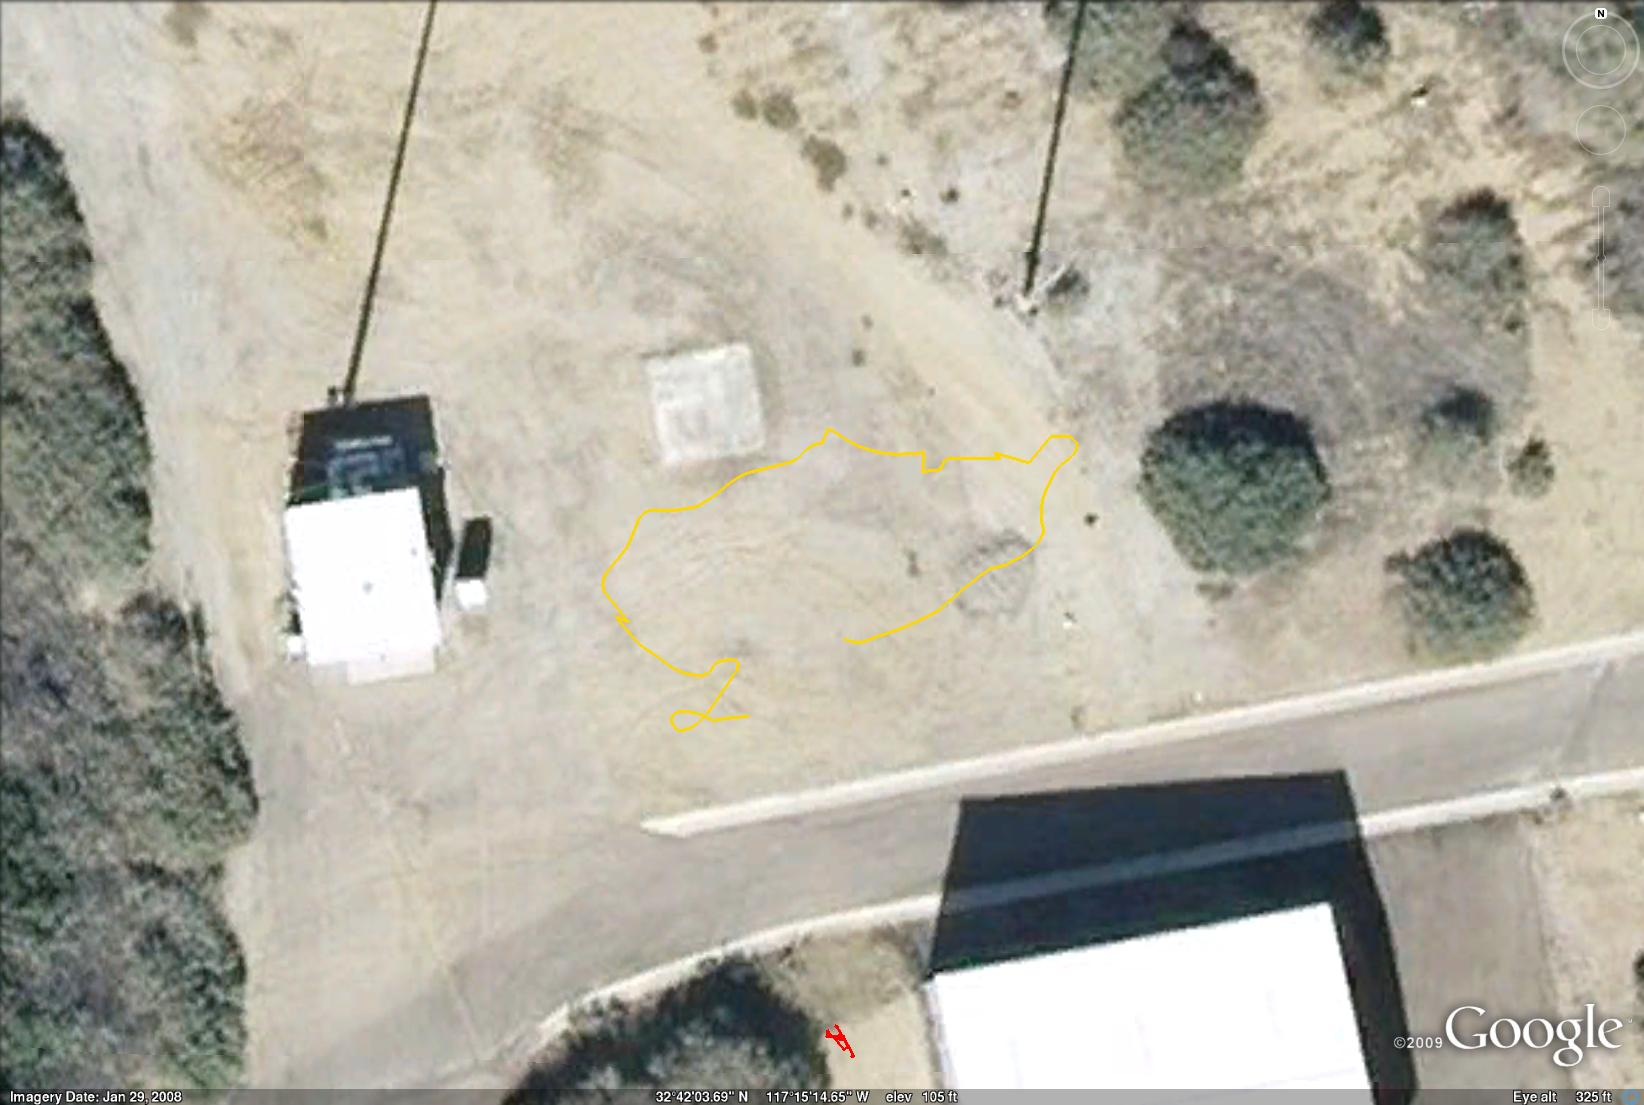
\includegraphics[width=.95\textwidth]{images/kfPlainDataFirstAttempt}
	\caption{Kalman filter output using the default parameters. The robot track is shown in yellow and a static GPS receiver with DGPS corrections is shown in red.}
	\label{fig:kfPlainDataFirstAttempt}
\end{figure}

\section{Lyapunov Controller Results}
\label{sec:lyapunovResults}
The control law derived in (\ref{eq:lyapunovControlLaw}) was tested in the previously described area and the results are shown in Figures \ref{fig:resultsLyapunovMocu} - \ref{fig:resultsLyapunovVelocities}. Figure \ref{fig:resultsLyapunovMocu} shows the route consisting of five waypoints that the robot was instructed to navigate and Figure \ref{fig:resultsLyapunovGEKF} shows the actual position of the robot during navigation. Of the options considered in section \ref{sec:lyapunovVariables} for setting the desired goal heading for each waypoint the experiment generating this data used $\theta^\star=\alpha$.

\begin{figure}[ht!]
	\centering
	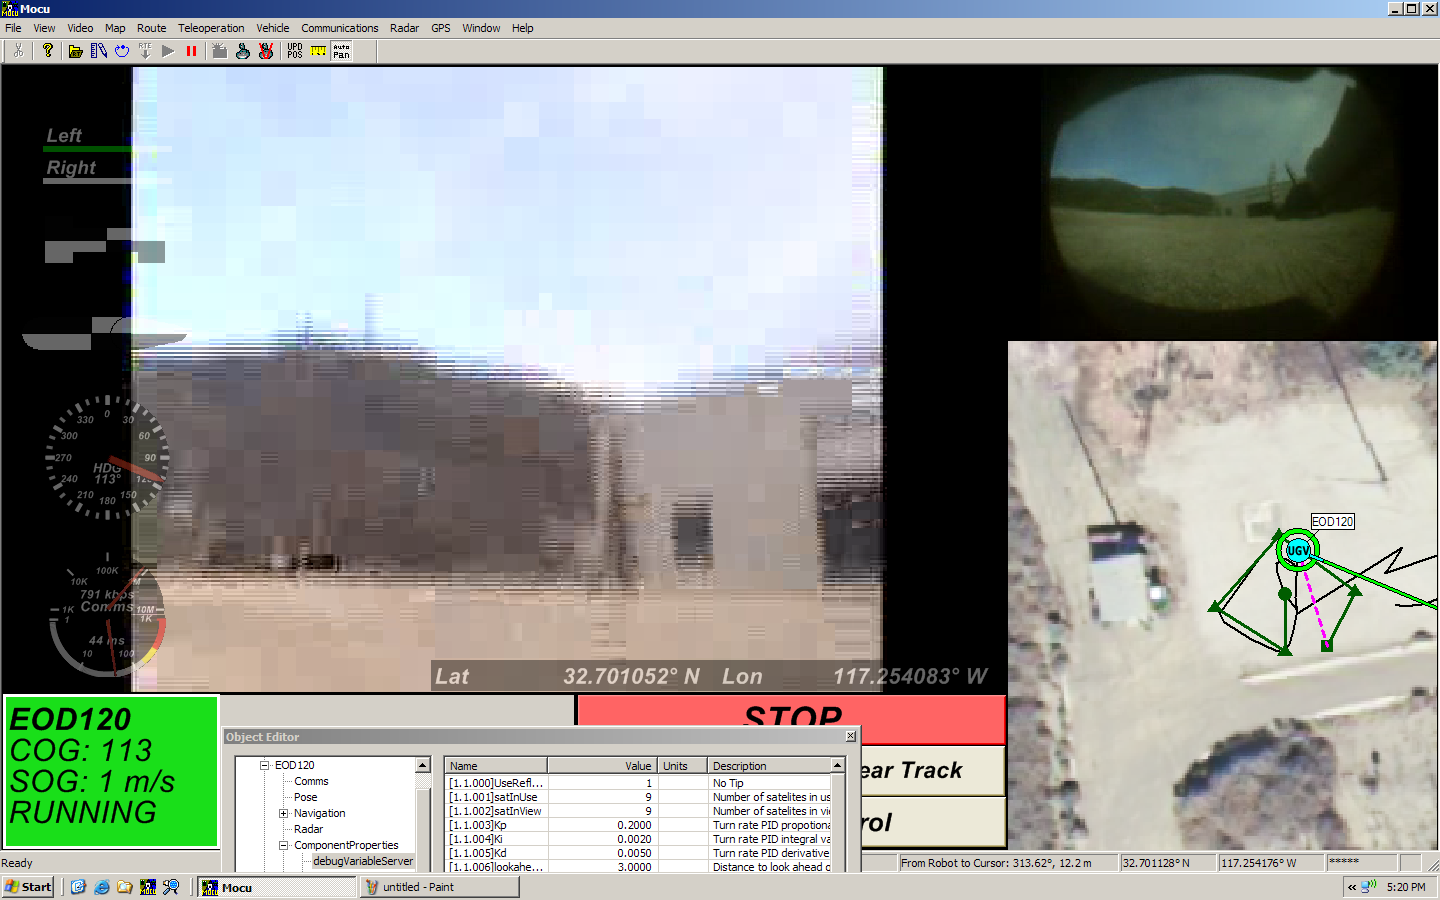
\includegraphics[width=.5\textwidth]{images/20100918_1717_mocu}
	\caption{Route generated using MOCU.}
	\label{fig:resultsLyapunovMocu}
\end{figure}

\begin{figure}[ht!]
	\centering
	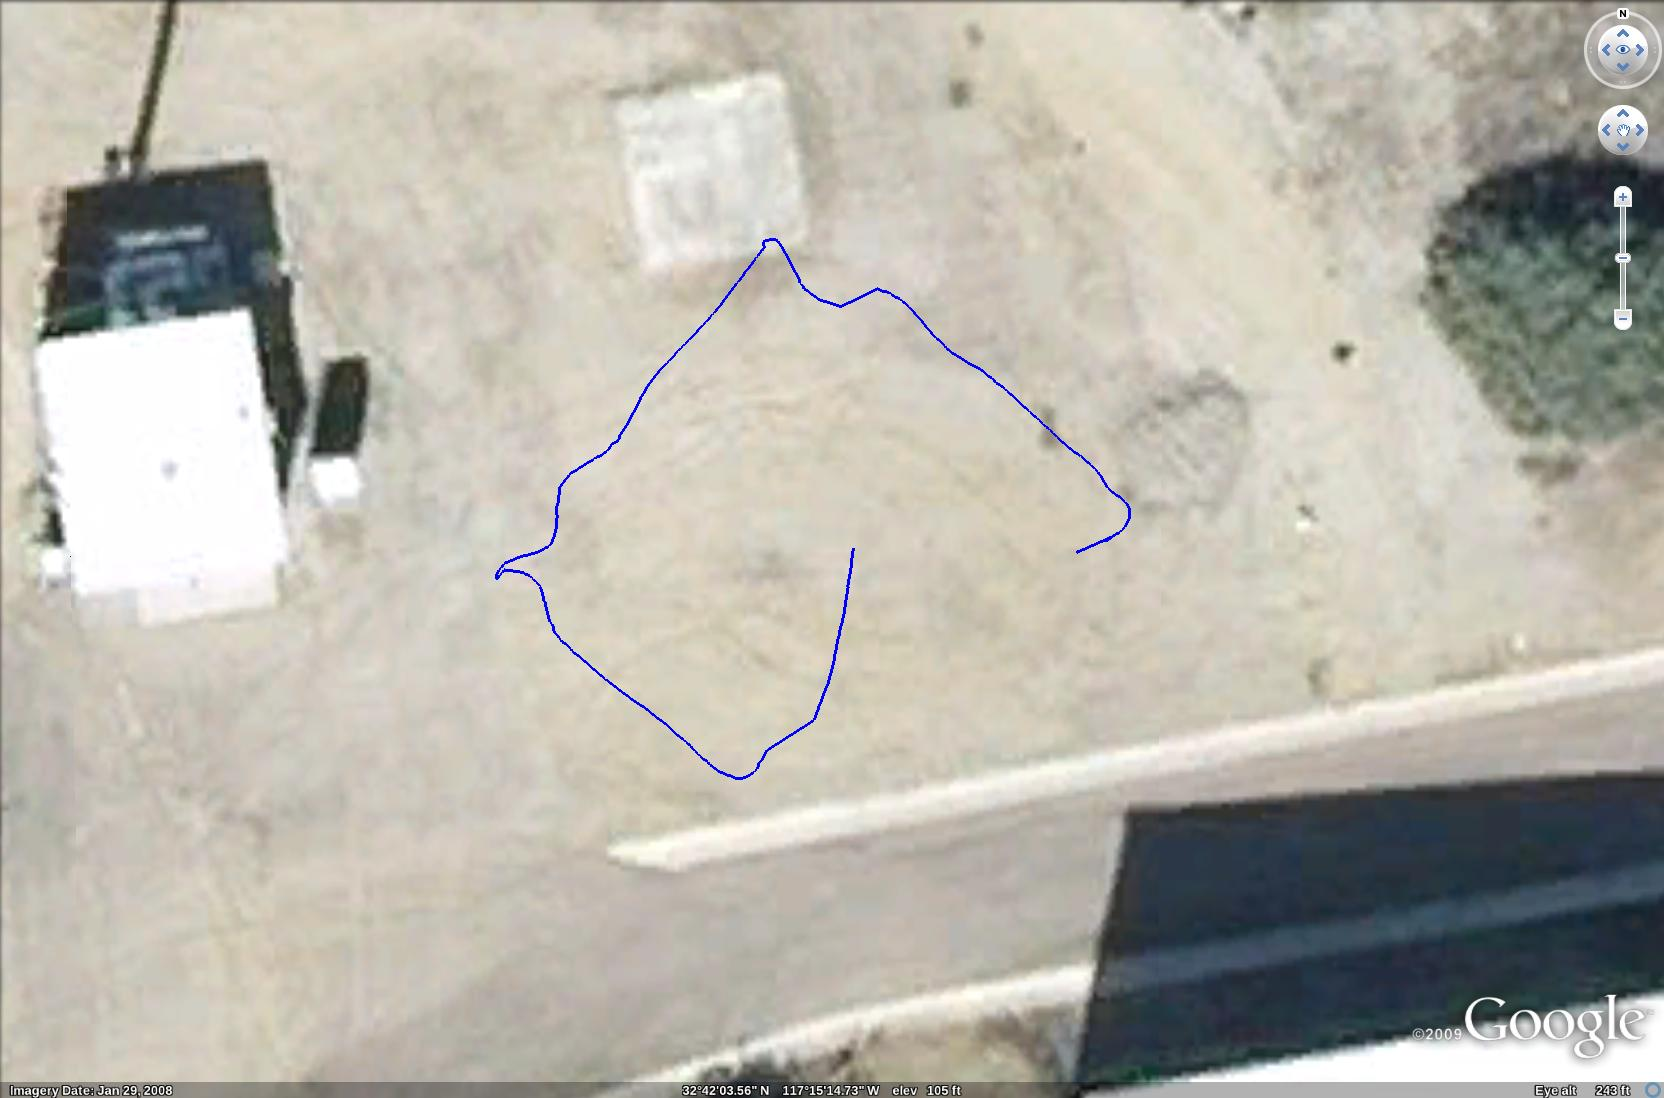
\includegraphics[width=.5\textwidth]{images/20100918_1717_GE_KF}
	\caption{Robot position during controller testing.}
	\label{fig:resultsLyapunovGEKF}
\end{figure}

Figure \ref{fig:resultsLyapunovVelocities} shows how the linear and angular velocities changed over time as measured by the Kalman filter output. The gains used were $h=0.1$, $k=0.25$ and $\gamma=0.23$. A clear deceleration can be seen as the robot approaches each waypoint although the linear velocity does not go to zero until the final waypoint due to the use of the carrot in the path planner as discussed in section \ref{sec:lyapunovVariables} for determing the error distance $e$. One of the consequences of using a model based controller is that a negative linear velocity was used after reaching the second waypoint and having the error angle $\alpha$ move towards the third waypoint which is rarely, if ever, encountered when using the original PID controller.

The results in this section show that the control law in (\ref{eq:lyapunovControlLaw}) using Lyapunov stability theory has the potential to provide a solution to the problem that the PID controller faced where the gains had to be tuned for different linear velocities since the model based controller has been shown to work when the goal heading and goal position are set arbitrarily. This will allow for improved navigation performance near obstacles.

\begin{figure}[ht!]
	\centering
	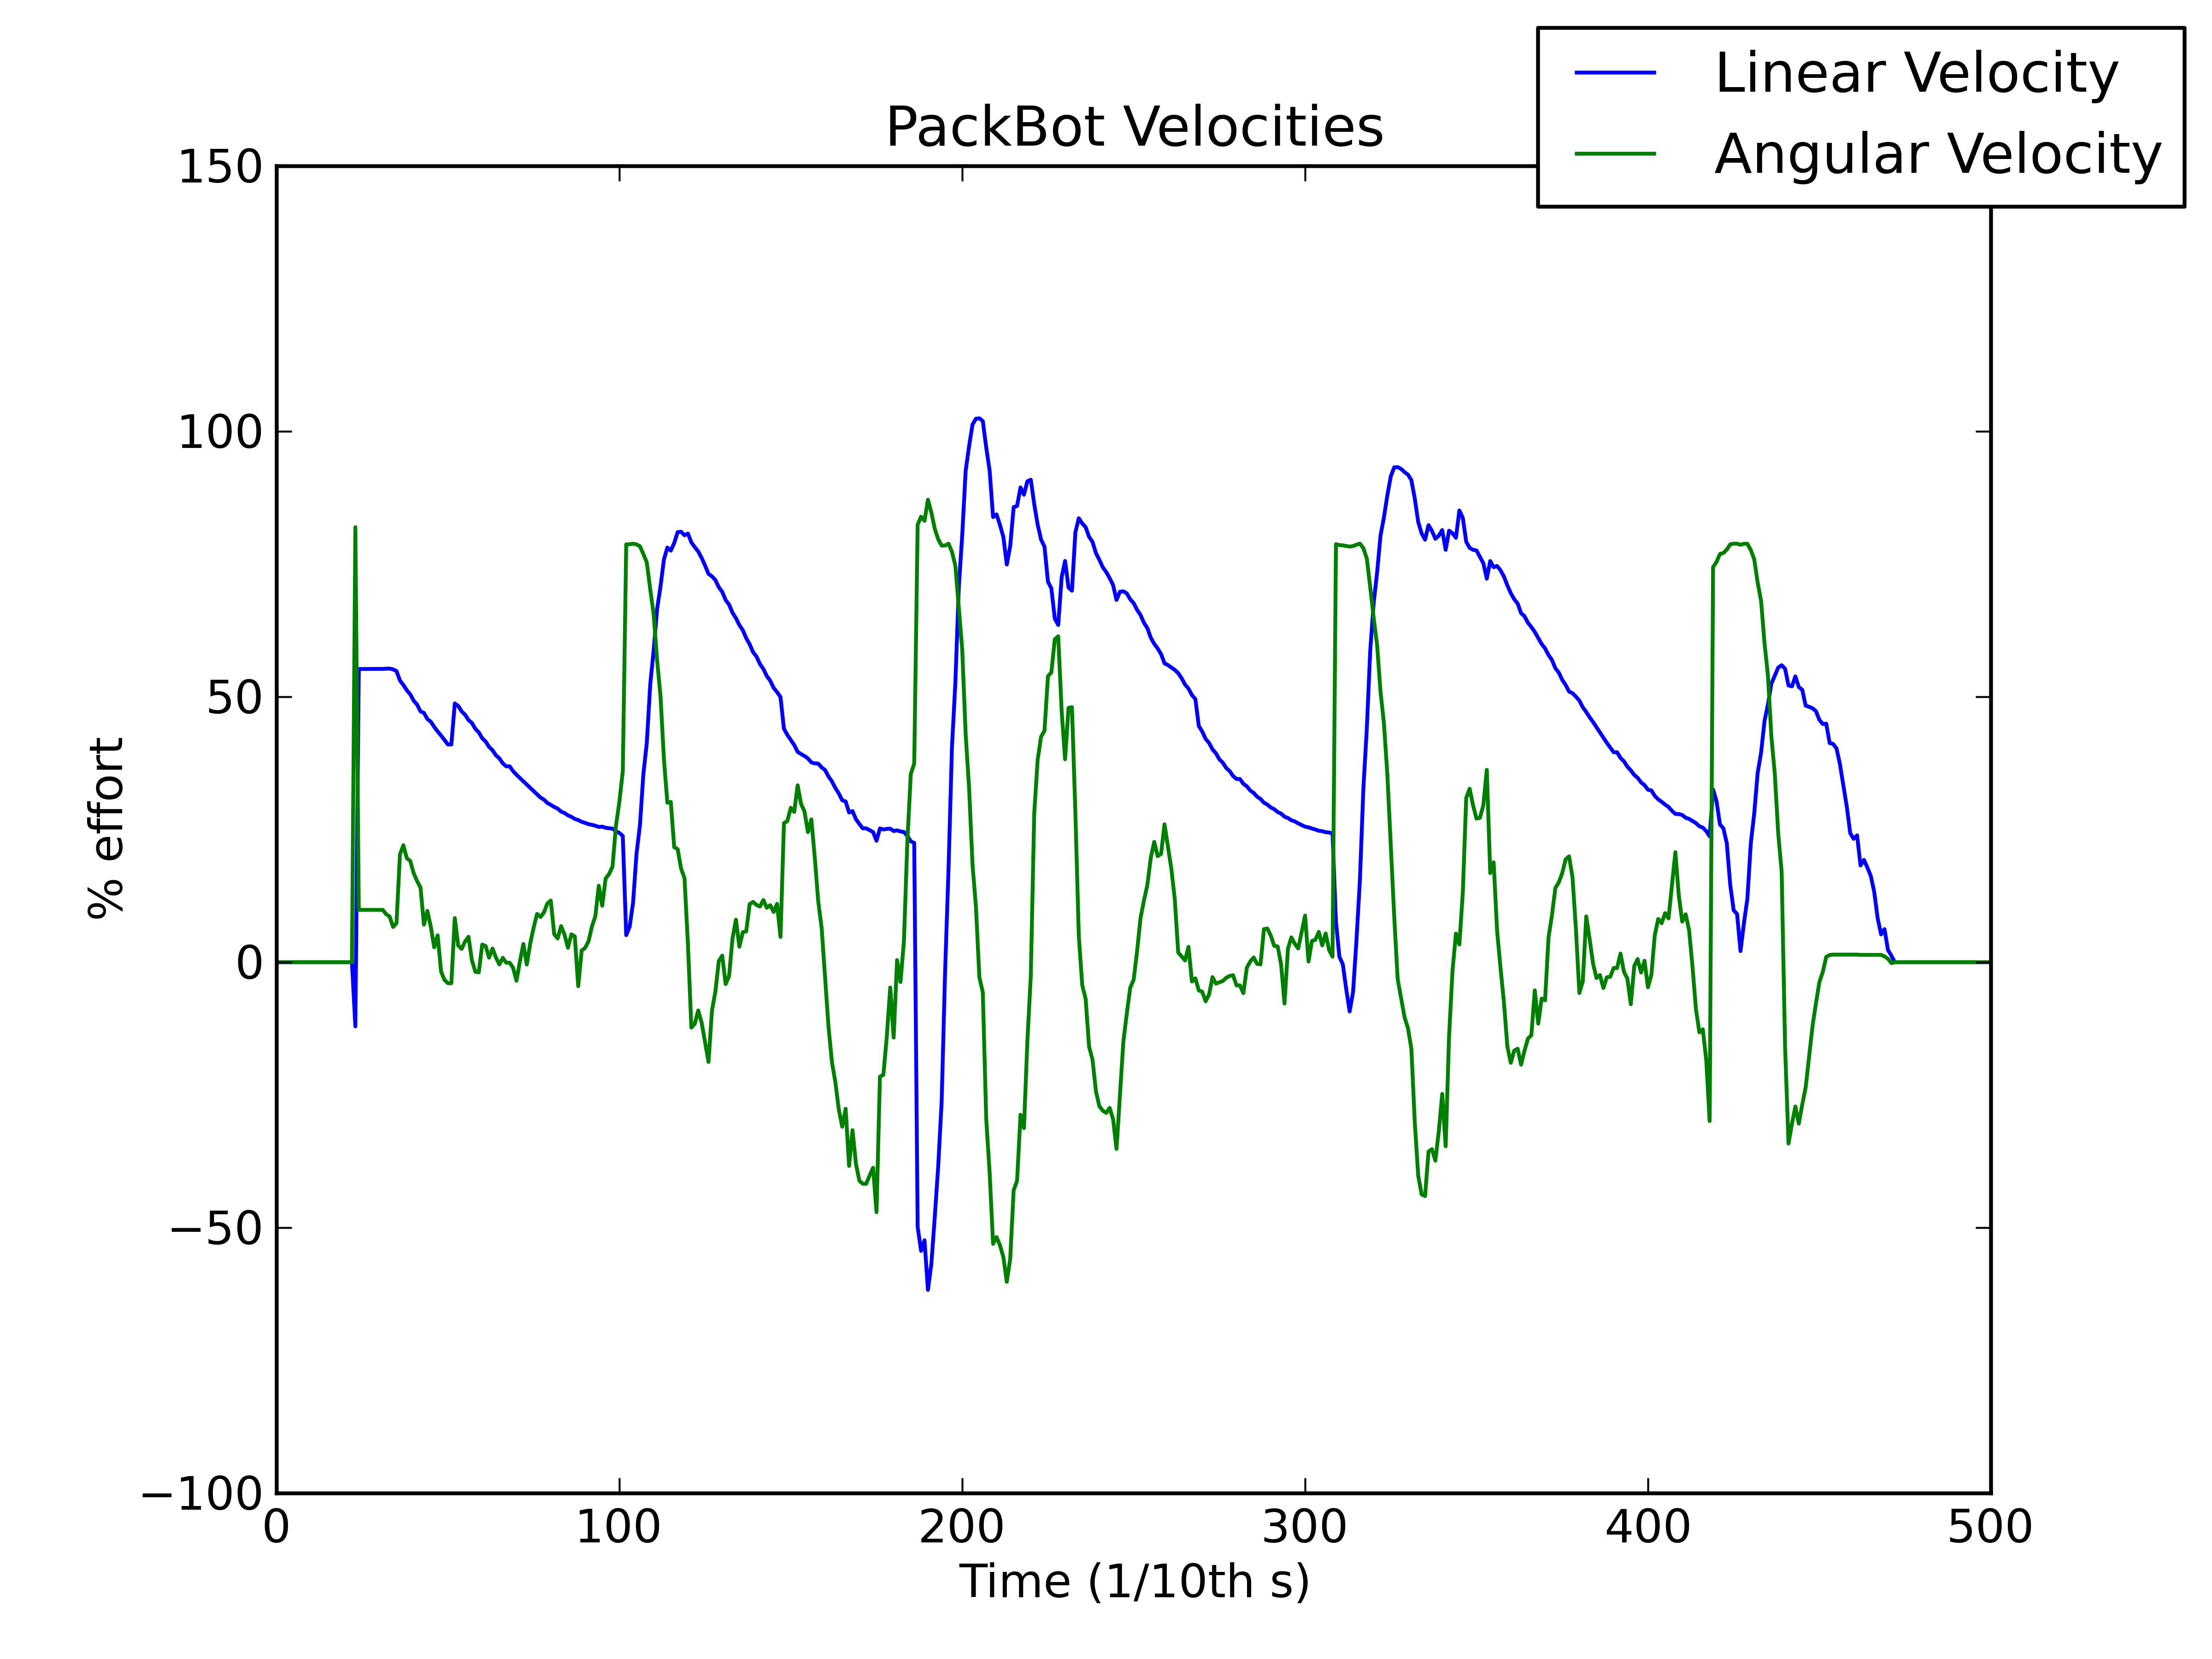
\includegraphics[width=.5\textwidth]{images/20100918_1717_velocities}
	\caption{Linear and angular velocity outputs using model based controller.}
	\label{fig:resultsLyapunovVelocities}
\end{figure}

\subsection{Controller Comparison}
\label{sec:controllerComparison}
*** Move Table \ref{tab:PIDGainEffects} here and make another table to show Lyapunov variables and how they affect curvature. Say that in both cases there are gains to tune but for PID they are tuned for stability whereas for Lyapunov stability is guaranteed and the gains only affect the curvature of the path. ***
